\chapter{试样加工与热处理实验}
\section{材料属性与试样加工过程}
\subsection{实验材料属性}
实验用的是真空自耗两次熔炼所得的钛合金板,其化学成分参数与室温(20℃)力学性能参数如\ref{sec:mytc4chem}与\ref{sec:mytc4machin}所示:
\begin{table}[htbp]
	\centering
	\caption{试样的化学成分参数}
	\label{sec:mytc4chem}
	\begin{tabular}{ccccccccc}
		\toprule
		元素($ \% $) & Al & V &Fe &C& O& N &H &其他杂质\\ \midrule
		实际含量 & 6.12&4.06 &0.13 &0.012&0.112&0.009&0.004 &$ \le 0.4 $ \\
		标准要求 &$ 5.5\sim 6.75 $ & $ 3.5\sim 4.5 $&$ \le 0.30 $ & $ \le 0.05 $&$ \le 0.20 $&$ \le 0.03$ &$ \le 0.015 $  & -- \\ \bottomrule
	\end{tabular}
\end{table}

\begin{table}[htbp]
	\centering
	\caption{试样的力学性能参数}
	\label{sec:mytc4machin}
	\begin{tabular}{cccc}
		\toprule
		力学性能& 抗拉强度$Mpa  $& 屈服强度$ Mpa $&断后伸长率$ \% $\\ \midrule
		实测值 & 983 &902 & 13\\
		标准值 &$ \ge 895 $&$ \ge 830 $&$ \ge 10 $ \\ \bottomrule
	\end{tabular}
\end{table}


为了节约成本,本设计选择了尺寸较小的试样来进行实验,整体尺寸为$ 25mm\times 7.5mm $的狗骨状片体,具体参数如\ref{fig:试样尺寸}所示:
%3-28日上午,经过老师说明,由于试样为板材,加工成圆柱较为困难,故加工成二位平面的“狗骨头”

\begin{figure}[h!]
	\centering
	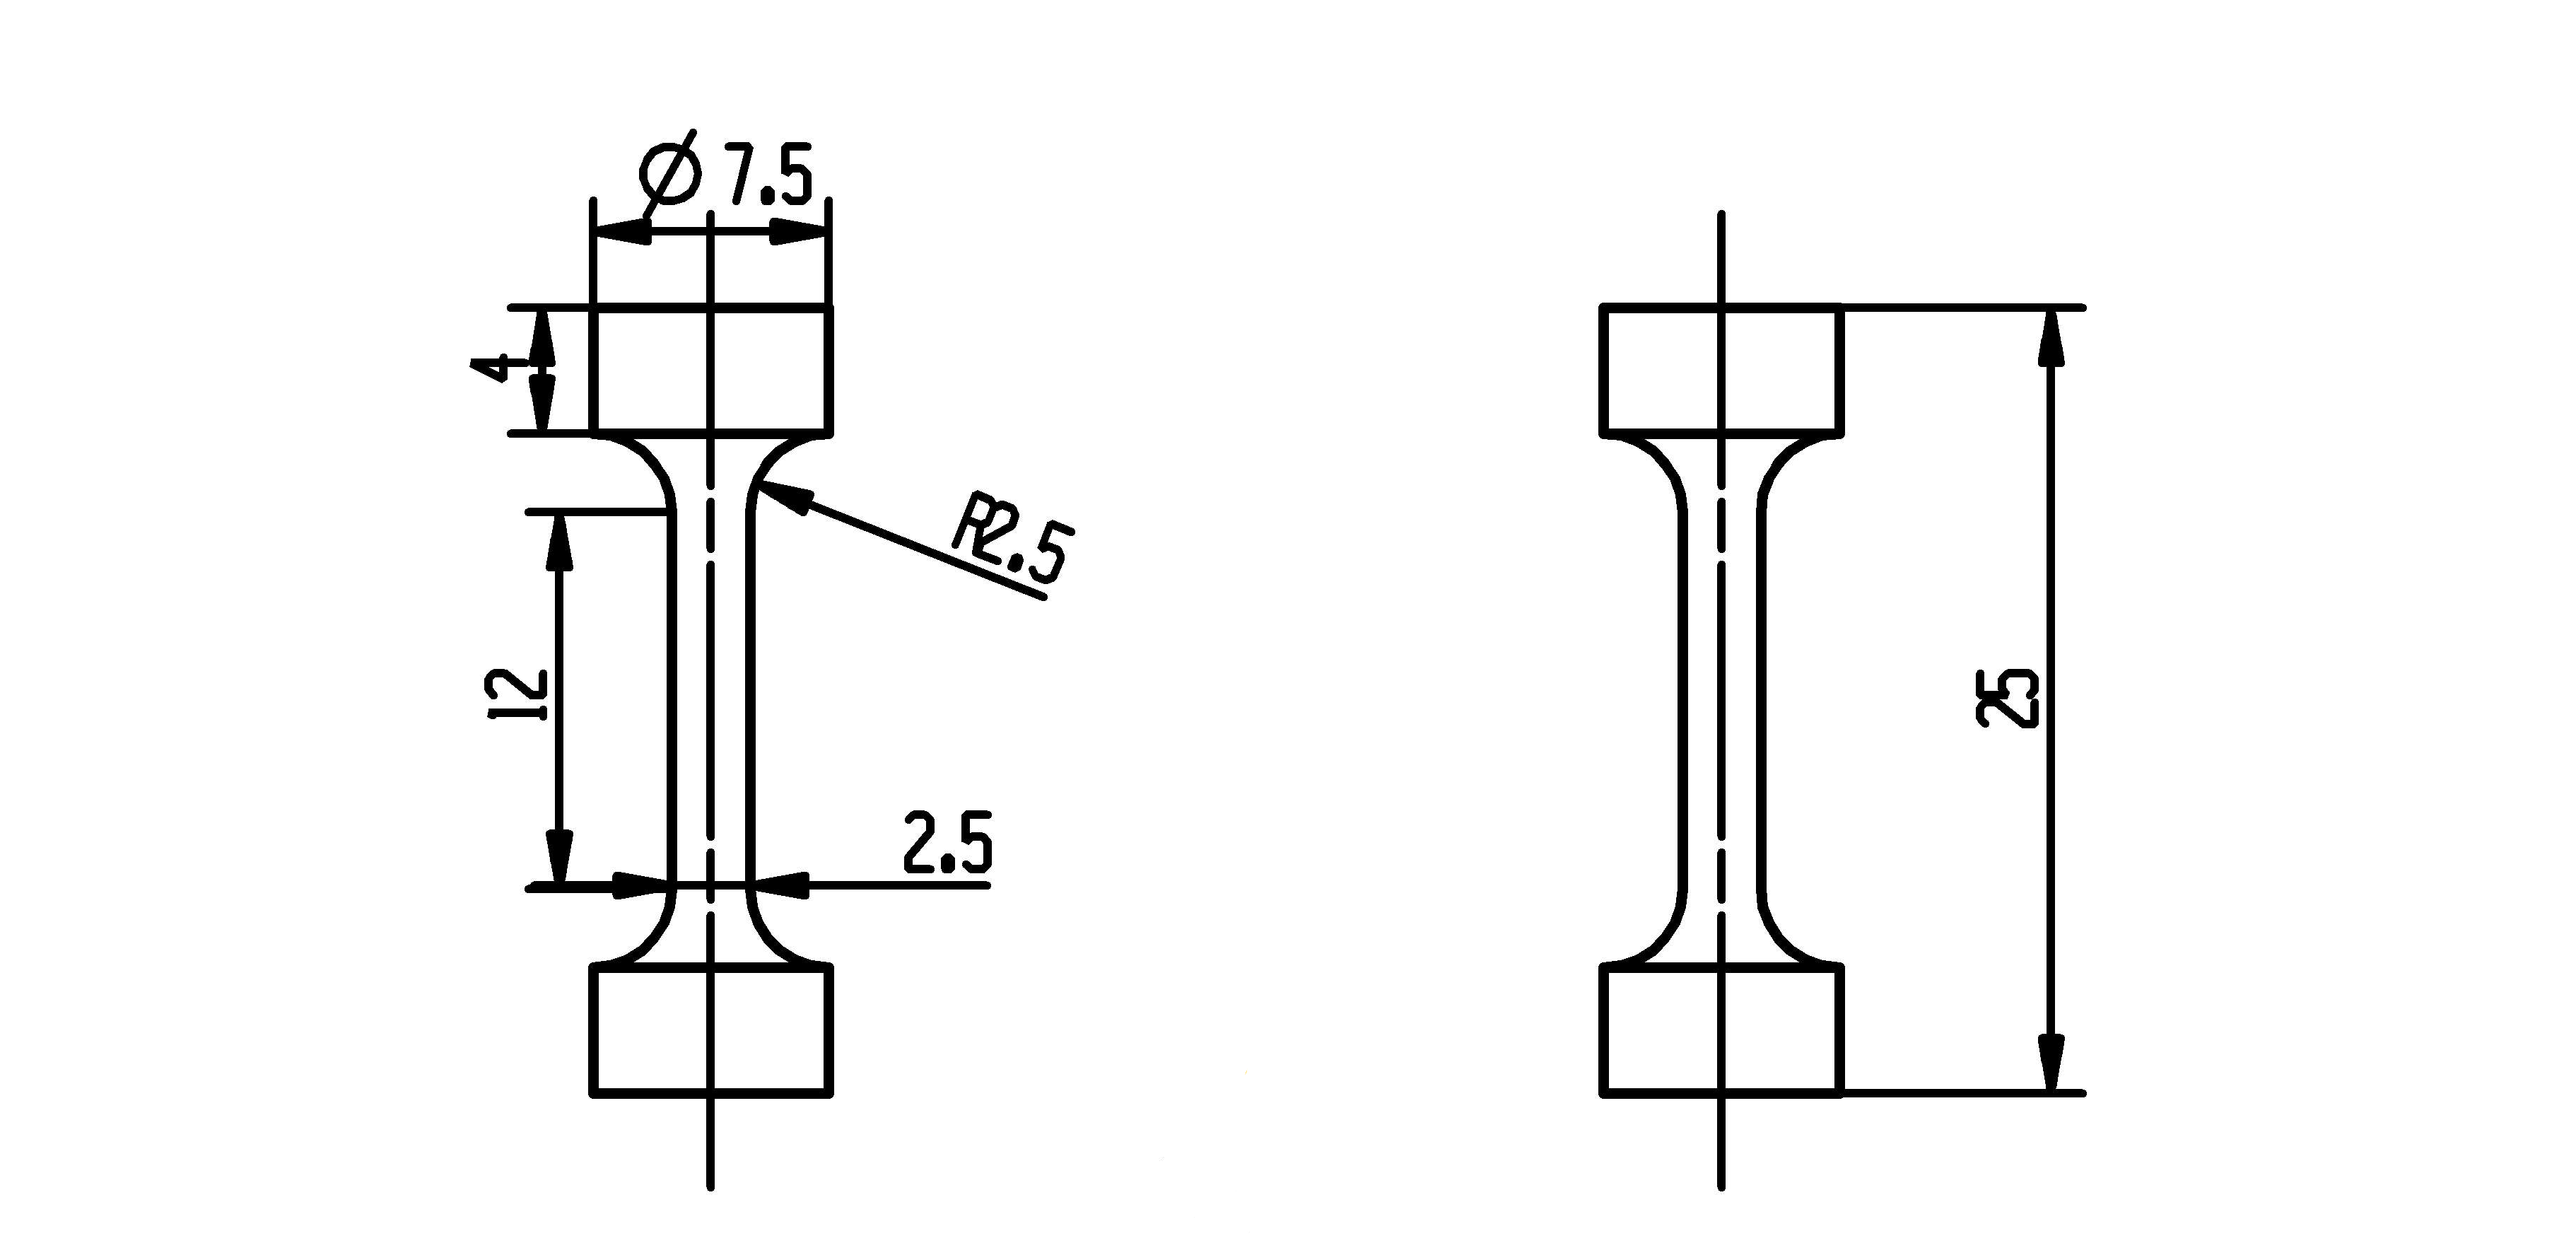
\includegraphics[width=0.99\linewidth]{pic/试样}
	\caption{试样的尺寸参数}
	\label{fig:试样尺寸}
\end{figure}

%
%\begin{figure}[!htbp]
%	\centering
%	\begin{minipage}[t]{0.68\textwidth}
	%		\centering
	%		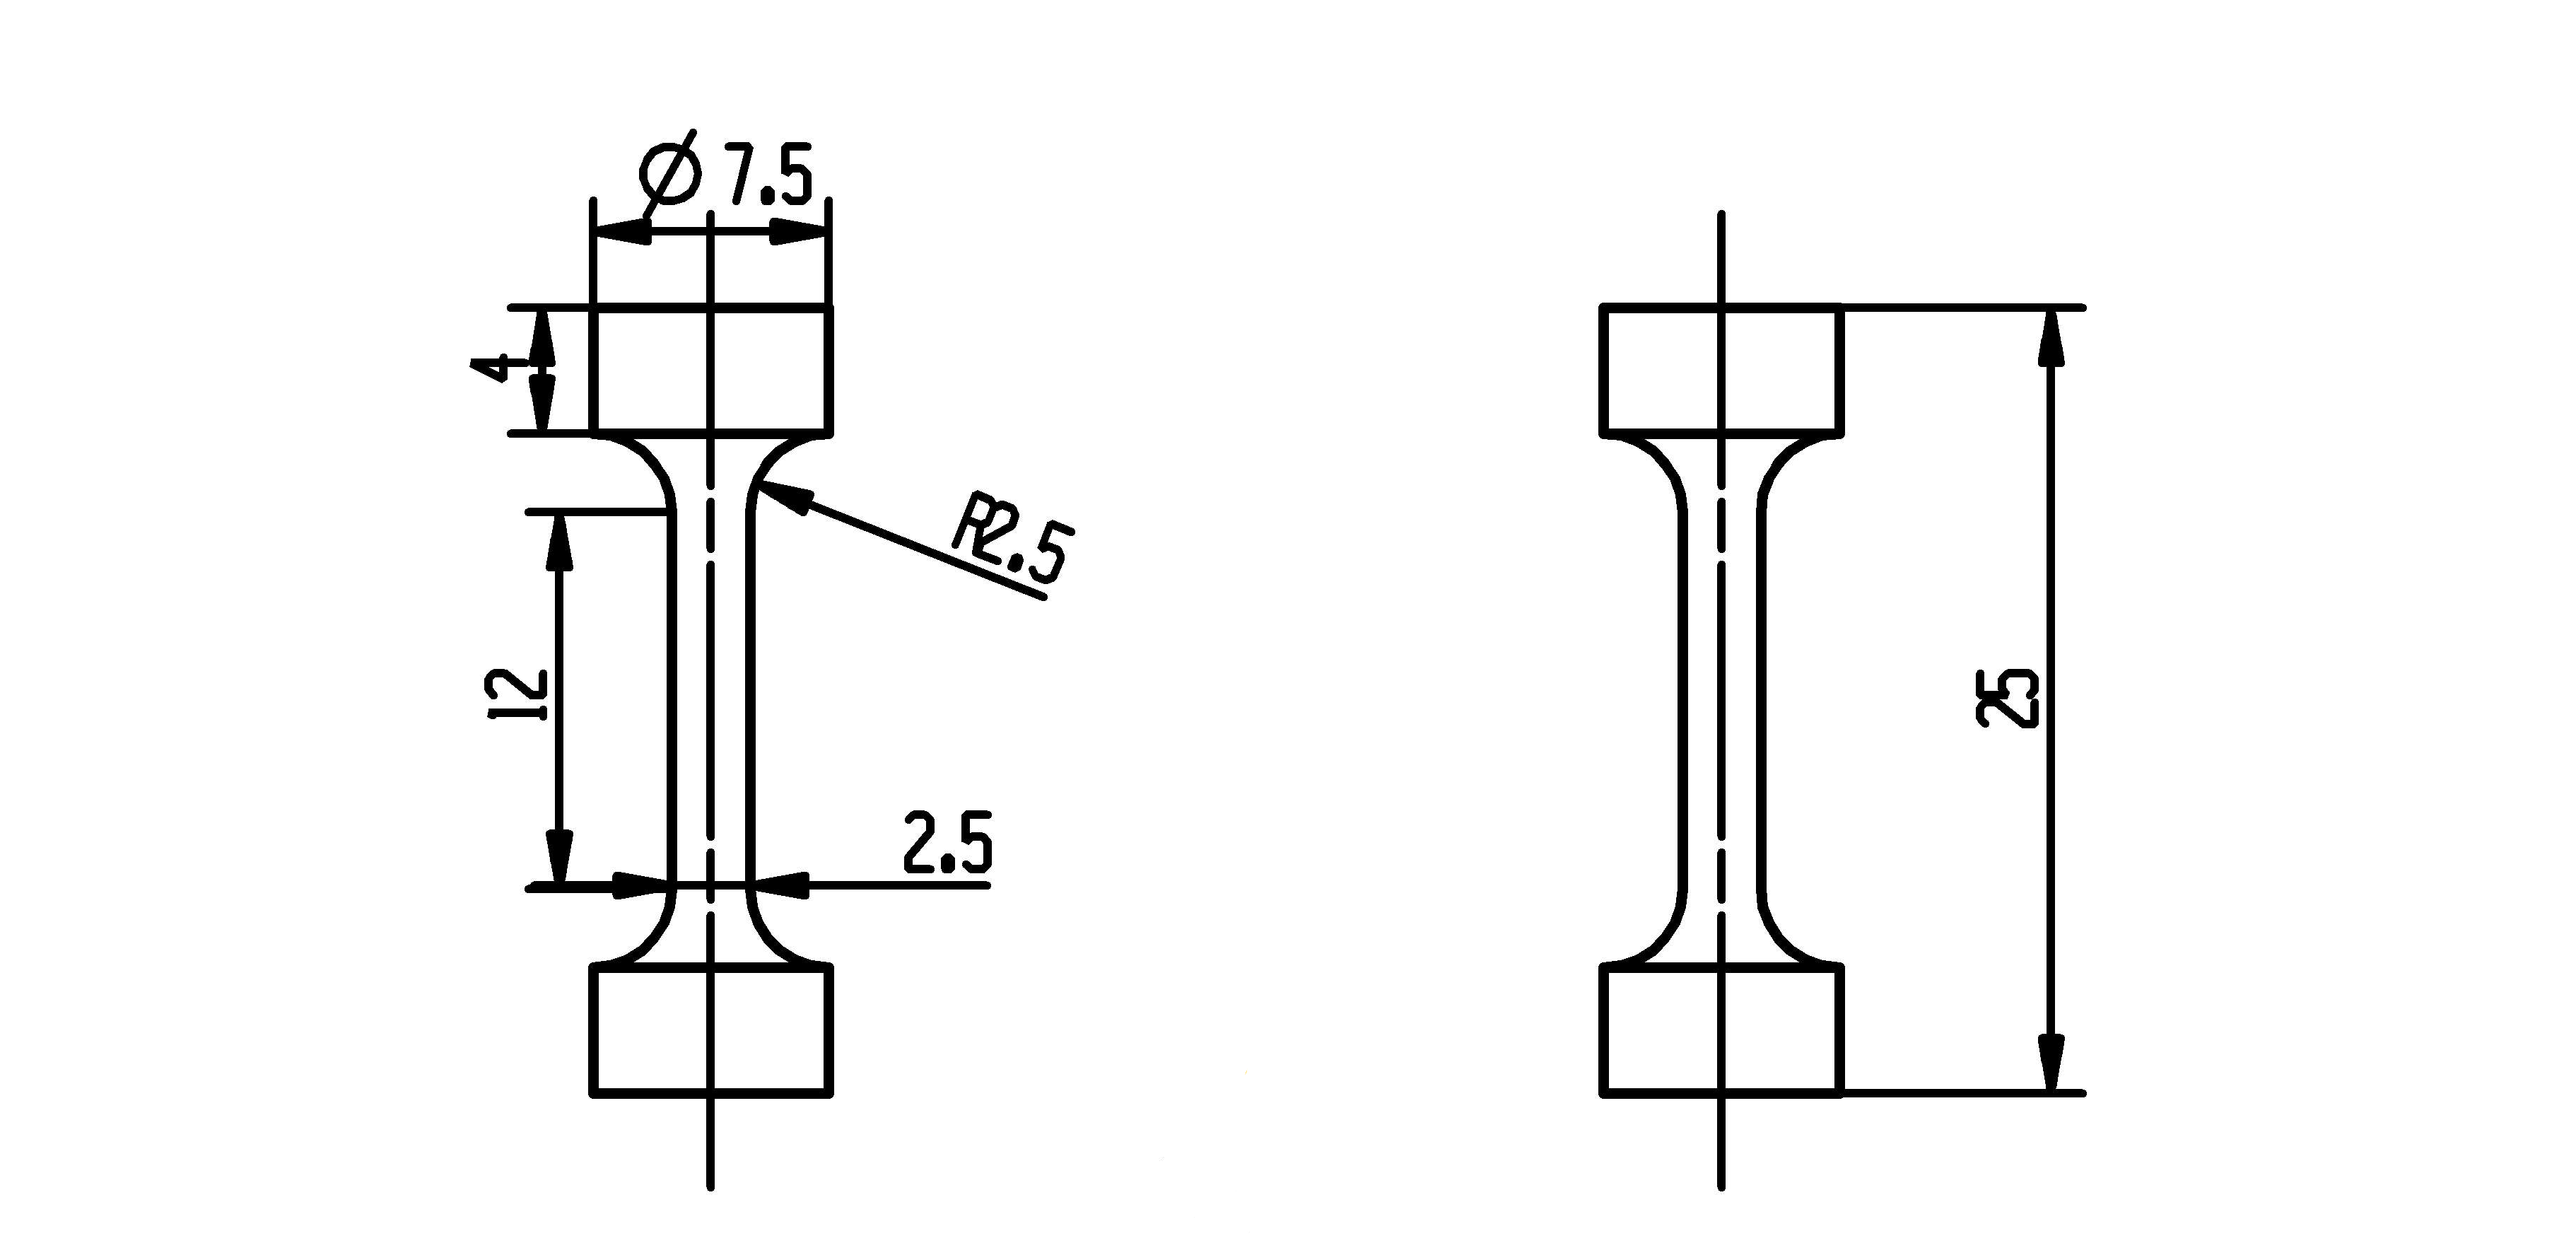
\includegraphics[width=6cm]{pic/试样}
	%		\caption{试样的尺寸参数}
	%		\label{fig:试样尺寸}
	%	\end{minipage}
%	\begin{minipage}[t]{0.3\textwidth}
	%		\centering
	%		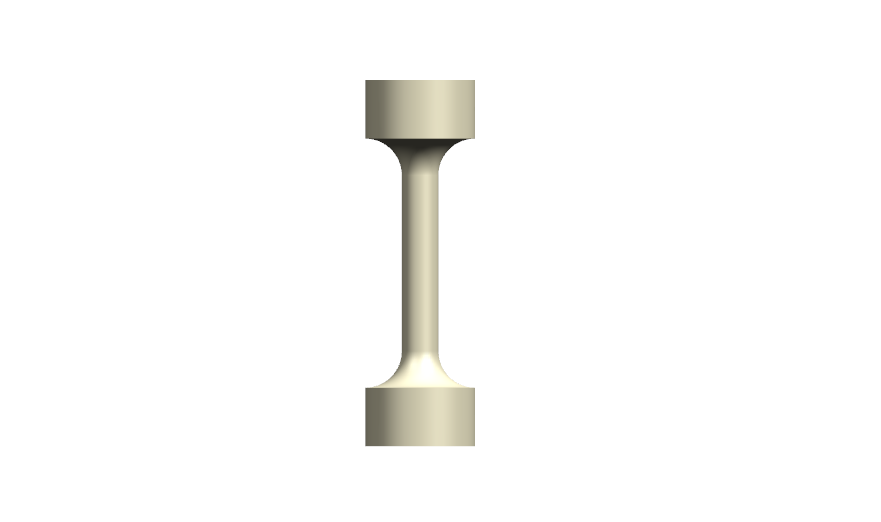
\includegraphics[width=6cm]{pic/模型}
	%		\caption{试样的三维模型}
	%		\label{fig:试样的三维模型}
	%	\end{minipage}
%%	\caption{试样参数}
%\end{figure}
\subsection{试样加工}
本设计采用电火花线切割加工(Wire cut Electrical Discharge Machining,简称WEDM)的方法进行加工。在一开始只考虑了材料的利用率,就设计了如\ref{fig:badway}所示的密集排列。但是在实际加工的时候,却发现在这样的设计方式根本不可行——没有夹具的位置,且刀路比较长。

\begin{figure}[h!]
	\centering
	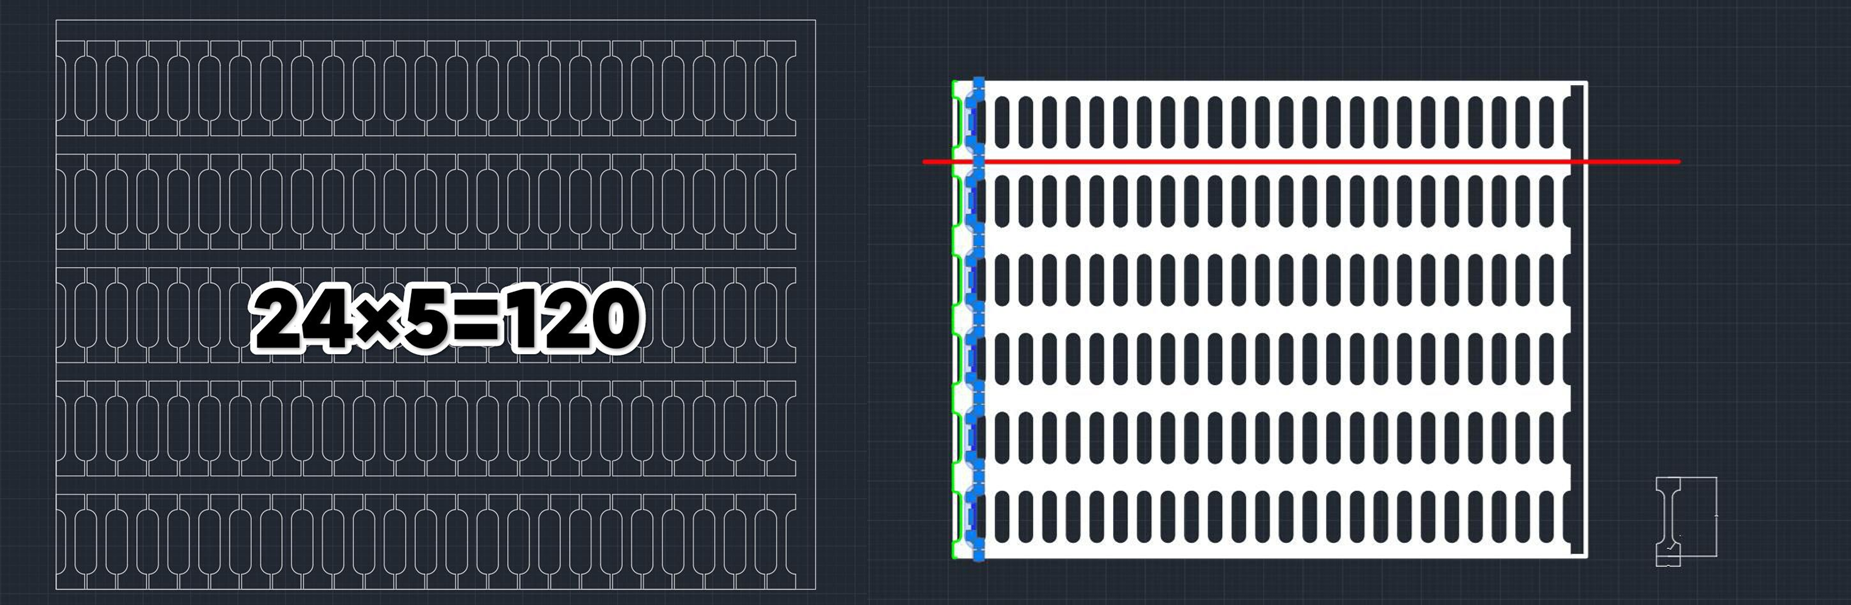
\includegraphics[width=0.8\linewidth]{pic/刀路初步}
	\caption{初步设计的刀路}
	\label{fig:badway}
\end{figure}


在仔细考虑了加工方法、设备特点、加工成本等因素后,在工程训练中心张冠老师的协助下,将加工方式改进成了:先把大板切割成八个小板,再把小板叠在一起进行加工。的方法,最终切割出来了$ 7\times 8=56 $个试样。
% TODO: \usepackage{graphicx} required
\begin{figure}[h!]
	\centering
	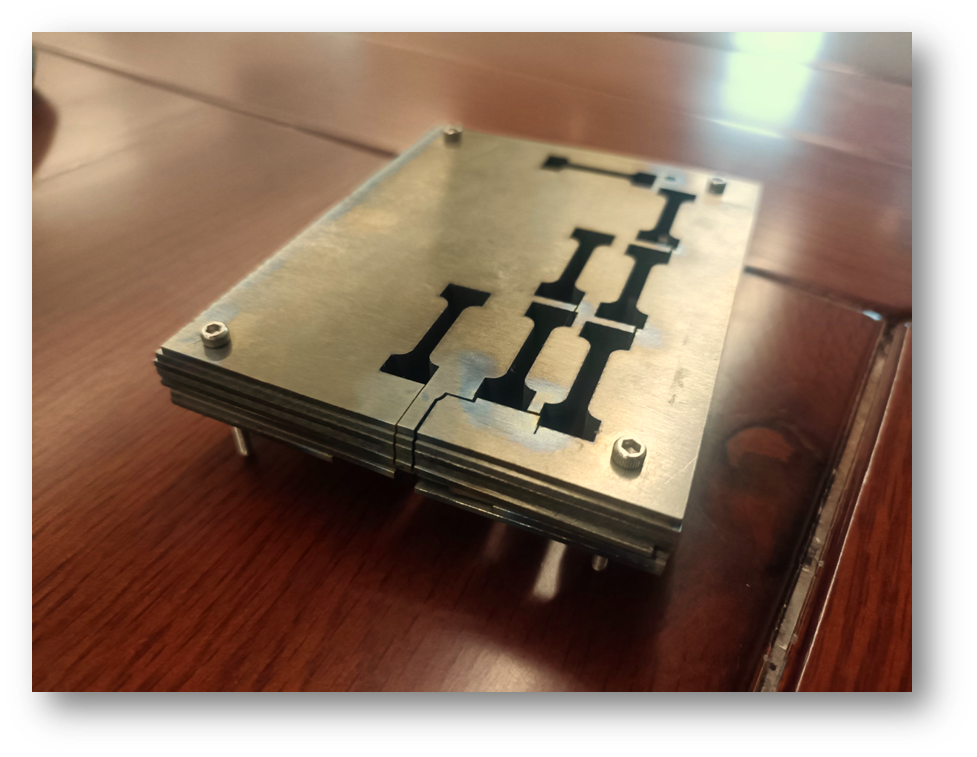
\includegraphics[width=0.7\linewidth]{pic/堆叠式切割}
	\caption{堆叠式切割}
	\label{fig:goodway}
\end{figure}


\section{TC4型钛合金的热处理工艺}
由~\ref{sec:1.1}可知,钛合金可以通过各种各样的相变过程来得到不同的组织结构。因而可以设计适宜的热处理工艺参数,来获得具有高强度的显微组织,由此实现\ti 合金力学性能和工艺性能的改善。\ti 合金热处理的一些特性如下:
\begin{enumerate}
%	\item 钛合金的热处理主要用于α+β型钛合金。因为对于纯α型钛合金而言,马氏体相变不会使钛合金的性能发生显著变化。只能依赖淬火形成的亚稳相(包括马氏体相)的时效分解来进行。
%	\item 热处理应该避免形成ω相。形成ω相会使钛合金变脆,正确选择时效工艺(例如,采用较高的时效温度)即可使相分解。
	\item α+β钛合金的淬透性差,淬火热应力大,淬火时零件易翘曲。由于导热性差,钛合金变形时易引起局部温升过高,使局部温度有可能超过β转变点而形成魏氏组织。
	\item 化学性质活泼。热处理时,钛合金易与氧和水蒸气反应,在工件表面形成具有一定深度的富氧层或氧化皮,使合金的性能降低。同时钛合金热处理时容易吸氢,引起氢脆。
	\item β转变点差异大。即使是同一成分,但由于冶炼炉次的不同,其β转变温度有时差别很大。
\end{enumerate}

常见的\ti 钛合金热处理工艺有:退火、淬火(往往加上时效处理)、形变热处理等,不同的热处理方式得到的组织性能各异。 鲁媛媛,马保飞等人研究发现在时效温度为450、500和550℃时初生α相的含量随温度升高逐渐增加;而在时效温度为600℃和650℃条件下初生α相含量因高温溶解而明显减少, β相尺寸相应增大。当时效温度为550℃时, 所得钛合金的显微组织最佳\cite{timing}。刘婉颖、林元华等人通过实验发现:在960 ℃/1 h + WQ进行固溶处理和500 ℃/4 h + AC下进行时效处理得到的\ti 具有最佳的力学性能\cite{960500};陈冠宇通过实验表明,在850℃进行退火处理时,在600℃进行时效处理可以使合金得到更好的耐腐蚀性能\cite{1200};李宸宇证明\ti 合金在900℃空冷固溶两小时在530℃时效四小时后具有更好的强硬度,而且固溶后冷速越快,合金的强硬度越高、塑韧性越差\cite{900}。%第46页


%不同热处理作用如下:
%\begin{enumerate}
%	\item 退火:用于提高合金塑形、稳定组织。
%	\item 淬火:用于强化组织,提高综合力学性能。
%	\item 形变热处理:与压力加工结合起来,同时发挥相变强化和热处理强化的作用。
%	\item 化学热强化:提高金属耐磨性,抗腐蚀性
%\end{enumerate}

%\subsection{热处理工艺对一般钛合金组织的影响}

\section{TC4钛合金的热处理方案设计}
对于α+β型的\ti 钛合金的固溶时效热处理工艺而言,其主要影响参数为温度和时间。在阅读了一些前人的研究报告\cite{mirror1}\cite{mirror2}之后,初步确定了固溶处理的最佳温度为$ \beta $相变点以下30℃左右处理一个小时、时效温度在450℃左右处理三个小时后,组织组成与综合力学性能最好,于是本设计首先确定了如下四个变量:固溶温度、固溶方式、时效温度、时效时间。
\subsection{正交实验设计}
用正交实验代替传统的控制变量法来提高实验效率、材料利用率。传统的控制变量法在面对低因素、低水平的实验时可以设计出很清晰直观的实验,但是面对多因素(变量)、多水平的实验时,控制变量法就显得极为繁琐了。比如一个含有三个变量,每个变量有三个水平的实验就需要$ 3\times 3 \times 3=27$次实验,为了直观性而牺牲大量的成本、同时包含了太多无关的对照组,这样的实验设计在很大程度上是不符合可持续发展理念的,是在浪费资源。但好在有另外一种方法可以解决问题——正交试验设计法(Orthogonal experimental design)。

正交实验设计是研究多因素多水平的又一种设计方法,它是根据正交性从全面试验中挑选出部分有代表性的点进行试验,这些有代表性的点具备了“均匀分散,齐整可比”的特点\cite{wangxueshen}。当实验次数太多时,根据正交实验设计,实验者可以选择一部分有代表性水平组合进行试验。 例如前面说的三因素三水平的实验,若按$ L9(3^4) $正交表安排实验,只需作9次,按$ L15(3^7) $正交表进行15次实验,显然大大减少了工作量。

在没有通过正交实验设计之前,笔者的实验是如\ref{sec:first}这样设置的:
\begin{table}[htbp]
	\centering
	\caption{\ti 原本的热处理制度设计}
	\label{sec:first}
	\begin{tabular}{cccccc}
		\toprule
		固溶温度/℃ &处理时间/h & 冷却方法 & 时效温度/℃  &处理时间/h & 冷却方法 \\
		\midrule
			910 & 1 & $\mathrm{WQ}$ & 510 & 4 & $\mathrm{AC}$\\
			910 & 1 & $\mathrm{FC}$  & 510 & 4 & $\mathrm{AC}$ \\
			910 & 1 & $\mathrm{WQ}$ & 550 & 4 & $\mathrm{AC}$ \\
			910 & 1 & $\mathrm{FC}$  & 550 & 4 & $\mathrm{AC}$ \\
			910 & 1 & $\mathrm{WQ}$ & 590 & 4 & $\mathrm{AC}$ \\
			910 & 1 & $\mathrm{FC}$  & 590 & 4 & $\mathrm{AC}$ \\
			\midrule
			950 & 1 & $\mathrm{WQ}$ & 510 & 4 & $\mathrm{AC}$ \\
			950 & 1 & $\mathrm{FC}$ & 510 & 4 & $\mathrm{AC}$ \\
			950 & 1 & $\mathrm{WQ}$ & 550 & 4 & $\mathrm{AC}$ \\
			950 & 1 & $\mathrm{FC}$ & 550 & 4 & $\mathrm{AC}$ \\
			950 & 1 & $\mathrm{WQ}$ & 590 & 4 & $\mathrm{AC}$ \\
			950 & 1 & $\mathrm{FC}$ & 590 & 4 & $\mathrm{AC}$ \\
			\midrule
			990 & 1 & $\mathrm{WQ}$ & 510 & 4 & $\mathrm{AC}$ \\
			990 & 1 & $\mathrm{FC}$ & 510 & 4 & $\mathrm{AC}$ \\
			990 & 1 & $\mathrm{WQ}$ & 550 & 4 & $\mathrm{AC}$ \\
			990 & 1 & $\mathrm{FC}$ & 550 & 4 & $\mathrm{AC}$ \\
			990 & 1 & $\mathrm{WQ}$ & 590 & 4 & $\mathrm{AC}$ \\
			990 & 1 & $\mathrm{FC}$ & 590 & 4 & $\mathrm{AC}$ \\
		\bottomrule
	\end{tabular}
\end{table}

从\ref{sec:first}可见,如果按照控制变量法设计实验,则至少需要$3\times2\times3  =18$次实验,才能穷举完所有变量各个水平之间的关系。为了给子孙后代留下天蓝、地绿、水清的美丽家园\footnote{出自2022年6月5日,习近平致2022年六五环境日国家主场活动的贺信},本实验高举可持续发展理念伟大旗帜,并结合正交实验方法$\color{teal} L9.3.4 $对实验进行了优化。最终的热处理制度如下表所示\footnote{其中WQ表示水冷、FC表示炉冷、AC表示空冷。}
\begin{table}[htbp]
	\centering
	\caption{\ti 合金的热处理制度}
	\label{sec:myHT}
	\resizebox{\linewidth}{!}{
\begin{tabular}{ccccccc}
	\toprule
		实验编号&固溶温度/℃ &处理时间/h & 冷却方法 & 时效温度/℃  &处理时间/h & 冷却方法 \\
	\midrule
	1 & 910 & 1 & WQ & 510 & 1 & AC \\
	2 & 910 & 1 & FC & 590 & 2 & AC \\
	3 & 910 & 1 & WQ & 550 & 3 & AC \\
	4 & 950 & 1 & WQ & 590 & 3 & AC \\
	5 & 950 & 1 & FC & 550 & 1 & AC \\
	6 & 950 & 1 & WQ & 510 & 2 & AC \\
	7 & 990 & 1 & WQ & 550 & 2 & AC \\
	8 & 990 & 1 & FC & 510 & 3 & AC \\
	9 & 990 & 1 & WQ & 590 & 1 & AC \\
%	910 & 1 & $\mathrm{WQ}$ & 510 & 4 & $\mathrm{AC}$\\
%	910 & 1 & $\mathrm{FC}$  & 510 & 4 & $\mathrm{AC}$ \\
%	910 & 1 & $\mathrm{WQ}$ & 550 & 4 & $\mathrm{AC}$ \\
%	910 & 1 & $\mathrm{FC}$  & 550 & 4 & $\mathrm{AC}$ \\
%	910 & 1 & $\mathrm{WQ}$ & 590 & 4 & $\mathrm{AC}$ \\
%	910 & 1 & $\mathrm{FC}$  & 590 & 4 & $\mathrm{AC}$ \\
%	\midrule
%	950 & 1 & $\mathrm{WQ}$ & 510 & 4 & $\mathrm{AC}$ \\
%	950 & 1 & $\mathrm{FC}$ & 510 & 4 & $\mathrm{AC}$ \\
%	950 & 1 & $\mathrm{WQ}$ & 550 & 4 & $\mathrm{AC}$ \\
%	950 & 1 & $\mathrm{FC}$ & 550 & 4 & $\mathrm{AC}$ \\
%	950 & 1 & $\mathrm{WQ}$ & 590 & 4 & $\mathrm{AC}$ \\
%	950 & 1 & $\mathrm{FC}$ & 590 & 4 & $\mathrm{AC}$ \\
%	\midrule
%	990 & 1 & $\mathrm{WQ}$ & 510 & 4 & $\mathrm{AC}$ \\
%	990 & 1 & $\mathrm{FC}$ & 510 & 4 & $\mathrm{AC}$ \\
%	990 & 1 & $\mathrm{WQ}$ & 550 & 4 & $\mathrm{AC}$ \\
%	990 & 1 & $\mathrm{FC}$ & 550 & 4 & $\mathrm{AC}$ \\
%	990 & 1 & $\mathrm{WQ}$ & 590 & 4 & $\mathrm{AC}$ \\
%	990 & 1 & $\mathrm{FC}$ & 590 & 4 & $\mathrm{AC}$ \\
	\bottomrule
\end{tabular}
}
\end{table}

\subsection{正交实验分析方法}
经过正交实验方法设计的实验虽然节省了试验次数,但是不能兼顾直观性,因而我们需要专门的分析工具才能分析出来,不同变量之间的相关性。
\\

{\Huge \color{red} \textbf {待补充}}

\section{TC4钛合金的热处理方案实验过程}

\subsection{实验设备}
本次设计热处理实验所用的设备为\text{\color{teal}JC-MF12-30}型箱式电阻炉,外观如\ref{fig: mymuffle}所示,设备规格如\ref{sec:mymuffle}所示:


\begin{table}[htbp]
	\centering
	\caption{\text{\color{teal}JC-MF12-30}型箱式电阻炉的规格}
	\label{sec:mymuffle}
		\begin{tabular}{cc}
			\toprule
			参数&值\\
			\midrule
			型号&JC-MF12-30\\
			编号&803229\\
			电压&380V\\
			功率&12KW\\
			常用温度&1150℃\\
			最高温度&1200℃\\
			炉膛尺寸& 500$ \times $ 300$ \times $ 200(mm) \\
			制造日期&2023年2月\\
			制造商& $\text{青岛聚创}^\text{\textregistered}  $环保集团有限公司\\
			\bottomrule
		\end{tabular}
\end{table}

\begin{figure}[h!]
	\centering
	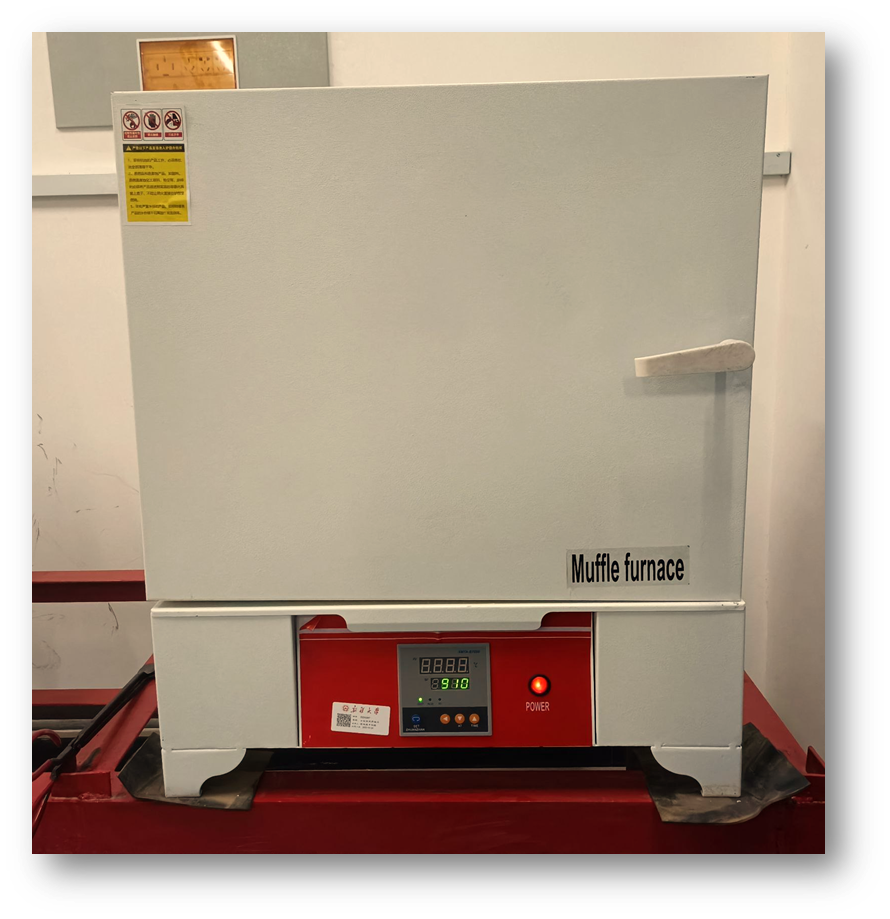
\includegraphics[width=0.7\linewidth]{pic/马弗炉}
	\caption{马弗炉外形}
	\label{fig: mymuffle}
\end{figure}

固溶实验需要淬火,用到的淬火液体如\ref{fig:淬火用液体}所示:
\begin{figure}[h!]
	\centering
	\subfigure[水淬液]{
		\label{fig:subfig:WCfluid}
		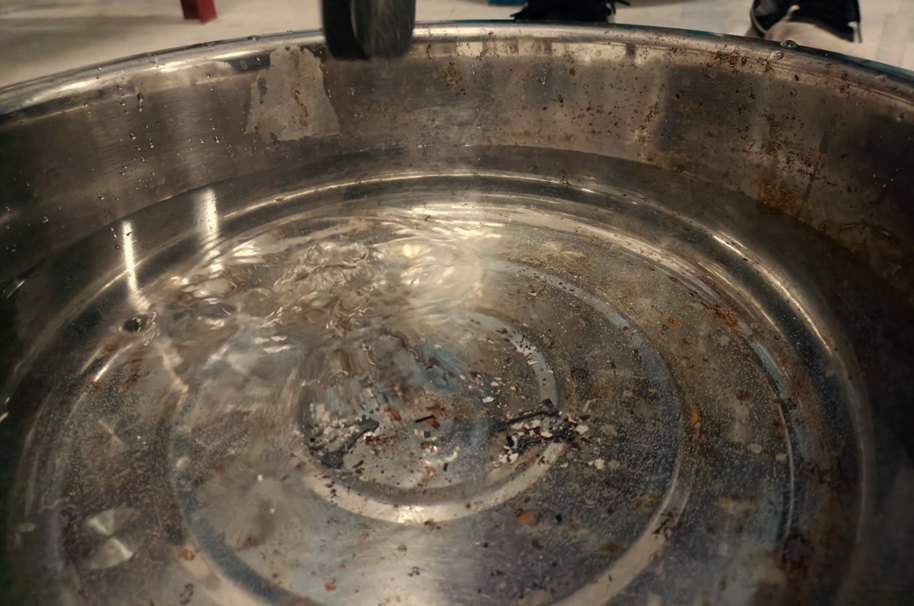
\includegraphics[scale=0.4]{pic/水淬液}}
	\hspace{0.5in} % 两图片之间的距离
	\subfigure[淬火油]{
		\label{fig:subfig:OCfluid}
		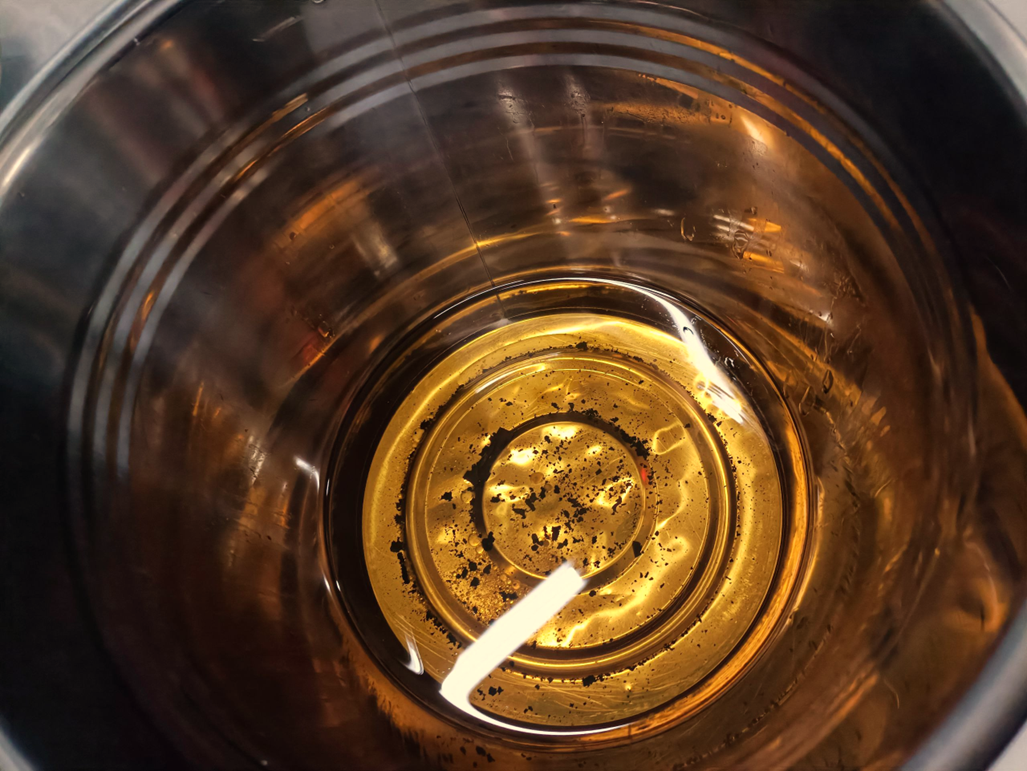
\includegraphics[scale=0.32]{pic/淬火油}}
	\caption{淬火用的液体}
	\label{fig:淬火用液体}
\end{figure}
\subsection{实验过程}
本次实验需要进行两次热处理——固溶与时效,基本步骤大同小异:
\begin{enumerate}
	\item 设定好预定的温度梯度与加热时间。
	\item 当温度到了预设值附近,戴好隔热手套,镊住式样,开炉门,快速准确放置好试样。
	\item 保温了足够时间后,开炉门,迅速夹取处理后的试样,并放入准备好的对应淬火液中。
	\item 擦拭淬火后的试样,处理表面脱落,归类试样。
\end{enumerate}

\section{小结}
